\begin{figure}[t]
\centering
\caption{Ablation under three judges (primary driver, five repetitions; error bars: bootstrap 95\% CI). Condition ordering varies across judges: the same-model judge ranks the full system below both ablations, the cross-vendor judge above both.}
\label{fig:flip}
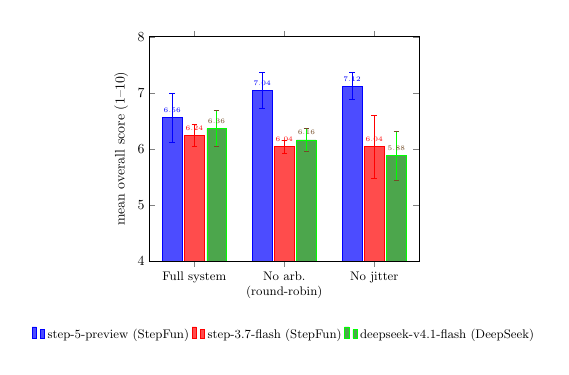
\begin{tikzpicture}[scale=0.50, transform shape]
\begin{axis}[
    ybar, bar width=14pt, ymin=4, ymax=8,
    ylabel={mean overall score (1--10)},
    symbolic x coords={full, rr, nj},
    xticklabels={Full system, No arb.\\ (round-robin), No jitter},
    xtick=data, x tick label style={align=center, font=\small}, ybar=2pt,
    enlarge x limits=0.25,
    legend style={at={(0.5,-0.28)}, anchor=north, legend columns=3, font=\small, draw=none},
    error bars/y dir=both, error bars/error bar style={thick},
    nodes near coords, every node near coord/.append style={font=\tiny, /pgf/number format/fixed, /pgf/number format/precision=2},
]
\addplot+[fill=blue!70, draw=blue, error bars/.cd, y explicit] coordinates {(full, 6.560) +- (0, 0.440) (rr, 7.040) +- (0, 0.320) (nj, 7.120) +- (0, 0.240)};
\addlegendentry{step-5-preview (StepFun)}
\addplot+[fill=red!70, draw=red, error bars/.cd, y explicit] coordinates {(full, 6.240) +- (0, 0.200) (rr, 6.040) +- (0, 0.120) (nj, 6.040) +- (0, 0.560)};
\addlegendentry{step-3.7-flash (StepFun)}
\addplot+[fill=green!50!black!70, draw=green, error bars/.cd, y explicit] coordinates {(full, 6.360) +- (0, 0.320) (rr, 6.160) +- (0, 0.200) (nj, 5.880) +- (0, 0.440)};
\addlegendentry{deepseek-v4.1-flash (DeepSeek)}
\end{axis}
\end{tikzpicture}
\end{figure}

\begin{figure}[t]
\centering
\caption{Per-discussion overall scores for all three judge pairs (32 discussions). Dashed line: perfect agreement. No pair shows tight agreement.}
\label{fig:trajectories}
\begin{tikzpicture}
\begin{groupplot}[group style={group size=3 by 1, horizontal sep=0.7cm},
    width=0.3\textwidth, height=0.24\textwidth,
    xmin=4, xmax=8, ymin=4, ymax=8,
    xtick={5,6,7,8}, ytick={5,6,7,8},
    grid=both, grid style={gray!20},
]
\nextgroupplot[xlabel={step-5-preview}, ylabel={step-3.7-flash}]
\addplot[only marks, mark=*, mark size=1.2pt, blue!70] coordinates {(7.40, 6.60) (7.00, 6.00) (6.40, 6.80) (6.60, 6.40) (7.00, 6.60) (6.60, 7.00) (7.80, 6.40) (6.20, 6.20) (6.60, 6.40) (7.00, 6.40) (6.20, 5.80) (7.20, 6.20) (5.80, 6.40) (7.20, 6.80) (7.40, 6.20) (7.20, 5.60) (6.60, 5.00) (7.20, 6.60) (7.40, 6.00) (6.60, 6.00) (7.20, 5.80) (7.40, 6.20) (6.60, 6.20) (6.00, 5.60) (6.20, 6.60) (6.20, 6.60) (4.80, 6.20) (6.20, 7.40) (6.80, 7.20) (6.60, 6.40) (6.60, 6.60) (7.20, 6.40)};
\addplot[dashed, gray, domain=4:8] {x};
\nextgroupplot[xlabel={step-5-preview}, ylabel={deepseek-v4.1-flash}]
\addplot[only marks, mark=*, mark size=1.2pt, blue!70] coordinates {(7.40, 5.80) (7.00, 5.40) (6.40, 5.40) (6.60, 5.40) (7.00, 6.20) (6.60, 5.60) (7.80, 6.40) (6.20, 5.40) (6.60, 6.80) (7.00, 5.80) (6.20, 6.20) (7.20, 6.80) (5.80, 6.20) (7.20, 5.00) (7.40, 5.80) (7.20, 6.20) (6.60, 5.80) (7.20, 6.60) (7.40, 6.20) (6.60, 5.80) (7.20, 6.40) (7.40, 6.00) (6.60, 6.40) (6.00, 5.60) (6.20, 6.40) (6.20, 6.00) (4.80, 4.20) (6.20, 5.80) (6.80, 5.00) (6.60, 5.60) (6.60, 6.60) (7.20, 6.20)};
\addplot[dashed, gray, domain=4:8] {x};
\nextgroupplot[xlabel={step-3.7-flash}, ylabel={deepseek-v4.1-flash}]
\addplot[only marks, mark=*, mark size=1.2pt, blue!70] coordinates {(6.60, 5.80) (6.00, 5.40) (6.80, 5.40) (6.40, 5.40) (6.60, 6.20) (7.00, 5.60) (6.40, 6.40) (6.20, 5.40) (6.40, 6.80) (6.40, 5.80) (5.80, 6.20) (6.20, 6.80) (6.40, 6.20) (6.80, 5.00) (6.20, 5.80) (5.60, 6.20) (5.00, 5.80) (6.60, 6.60) (6.00, 6.20) (6.00, 5.80) (5.80, 6.40) (6.20, 6.00) (6.20, 6.40) (5.60, 5.60) (6.60, 6.40) (6.60, 6.00) (6.20, 4.20) (7.40, 5.80) (7.20, 5.00) (6.40, 5.60) (6.60, 6.60) (6.40, 6.20)};
\addplot[dashed, gray, domain=4:8] {x};
\end{groupplot}
\end{tikzpicture}
\end{figure}

\begin{figure}[t]
\centering
\caption{Same-machine replication (secondary driver, three repetitions; error bars: SD). Identical transcripts; only the judge differs. The driver's own model, a same-vendor sibling, and a cross-vendor judge produce three different condition orderings.}
\label{fig:samemachine}
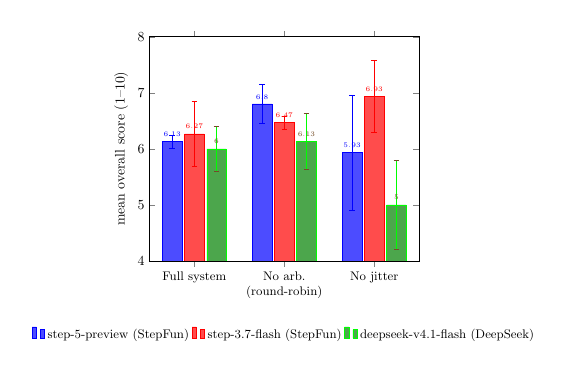
\begin{tikzpicture}[scale=0.50, transform shape]
\begin{axis}[
    ybar, bar width=14pt, ymin=4, ymax=8,
    ylabel={mean overall score (1--10)},
    symbolic x coords={full, rr, nj},
    xticklabels={Full system, No arb.\\ (round-robin), No jitter},
    xtick=data, x tick label style={align=center, font=\small}, ybar=2pt,
    enlarge x limits=0.25,
    legend style={at={(0.5,-0.28)}, anchor=north, legend columns=3, font=\small, draw=none},
    error bars/y dir=both, error bars/error bar style={thick},
    nodes near coords, every node near coord/.append style={font=\tiny, /pgf/number format/fixed, /pgf/number format/precision=2},
]
\addplot+[fill=blue!70, draw=blue, error bars/.cd, y explicit] coordinates {(full, 6.133) +- (0, 0.115) (rr, 6.800) +- (0, 0.346) (nj, 5.933) +- (0, 1.026)};
\addlegendentry{step-5-preview (StepFun)}
\addplot+[fill=red!70, draw=red, error bars/.cd, y explicit] coordinates {(full, 6.267) +- (0, 0.577) (rr, 6.467) +- (0, 0.115) (nj, 6.933) +- (0, 0.643)};
\addlegendentry{step-3.7-flash (StepFun)}
\addplot+[fill=green!50!black!70, draw=green, error bars/.cd, y explicit] coordinates {(full, 6.000) +- (0, 0.400) (rr, 6.133) +- (0, 0.503) (nj, 5.000) +- (0, 0.800)};
\addlegendentry{deepseek-v4.1-flash (DeepSeek)}
\end{axis}
\end{tikzpicture}
\end{figure}

\begin{figure}[t]
\centering
\caption{Speaking-count inequality (Gini over all three agents, zero-speech agents included) per ablation condition, both drivers.}
\label{fig:mechanism}
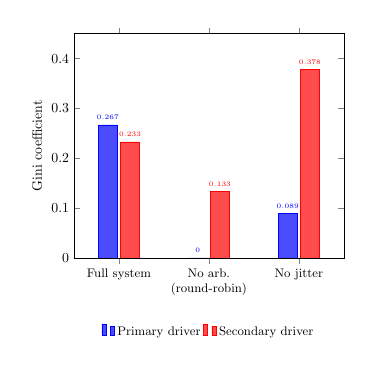
\begin{tikzpicture}[scale=0.50, transform shape]
\begin{axis}[
    ybar, bar width=14pt, ymin=0, ymax=0.45,
    ylabel={Gini coefficient},
    symbolic x coords={full, rr, nj},
    xticklabels={Full system, No arb.\\ (round-robin), No jitter},
    xtick=data, x tick label style={align=center, font=\small}, ybar=2pt,
    enlarge x limits=0.25,
    legend style={at={(0.5,-0.28)}, anchor=north, legend columns=2, font=\small, draw=none},
    nodes near coords, every node near coord/.append style={font=\tiny, /pgf/number format/fixed, /pgf/number format/precision=3},
]
\addplot+[fill=blue!70, draw=blue] coordinates {(full, 0.267) (rr, 0.000) (nj, 0.089)};
\addlegendentry{Primary driver}
\addplot+[fill=red!70, draw=red] coordinates {(full, 0.233) (rr, 0.133) (nj, 0.378)};
\addlegendentry{Secondary driver}
\end{axis}
\end{tikzpicture}
\end{figure}
